\documentclass[conference]{IEEEtran}

\ifCLASSINFOpdf

\else

\fi

% correct bad hyphenation here
\hyphenation{op-tical net-works semi-conduc-tor}

\usepackage{graphicx}
\usepackage{todonotes}
\usepackage{booktabs}


\begin{document}

%
% paper title
% Titles are generally capitalized except for words such as a, an, and, as,
% at, but, by, for, in, nor, of, on, or, the, to and up, which are usually
% not capitalized unless they are the first or last word of the title.
% Linebreaks \\ can be used within to get better formatting as desired.
% Do not put math or special symbols in the title.
\title{Architekturdokumentation\\Mensch \"argere Dich nicht!}


% author names and affiliations
% use a multiple column layout for up to three different
% affiliations
\author{\IEEEauthorblockN{Martin Puse}
\IEEEauthorblockA{
853001}
\and
\IEEEauthorblockN{Marcel Pillich}
\IEEEauthorblockA{863121}
}

% make the title area
\maketitle

% As a general rule, do not put math, special symbols or citations
% in the abstract
\begin{abstract}
Die vorliegende Arbeit enth\"alt eine detaillierte Beschreibung eines Prototypen einer Java-Applikation des Spiels "Mensch \"argere Dich nicht",
welche f\"ur Spieleprogrammierer und Spieledesigner gleicherma\ss en geeignet ist. Ziel war es, dass der Programmierer
sich um Erscheinungsbild und Regelumsetzung des Spiels k\"ummern kann, ohne selber Spielfelder designen zu m\"ussen, wohingegen der Designer keine
Programmierkenntnisse ben\"otigt, um neue Spielfelder hinzuzuf\"ugen und zu testen.\\ Zu diesem Zweck wurden eine Grammatik f\"ur die Spielfelder
und ein Generator, welcher die Grammatiken verarbeitet und automatisiert Code erzeugt, erstellt. Die dahinterliegende Idee, die Spielfelder
nicht auf Positions-, sondern Knoteninformationen zu basieren, wird ausf\"uhrlich dargestellt. Schlussendlich wird noch ein Abriss aller Komponenten der Architektur gegeben und erlangte Erkenntnisse dargelegt.
\end{abstract}

\IEEEpeerreviewmaketitle


\section{Einleitung}
% no \IEEEPARstart
"Mensch \"argere Dich nicht" ist ein Brettspiel f\"ur bis zu 4 Personen. Es z\"ahlt zu den Klassikern im deutschsprachigen Raum und wurde 1907/1908 von Josef Friedrich Schmidt in Anlehnung an das englische Spiel Ludo erfunden, die Urspr\"unge finden sich jedoch im indischen Spiel Pachisi. Erstmals 1910 erschienen ging es 1914 in Serie. 
\begin{figure}[]
    \centering
    \fbox{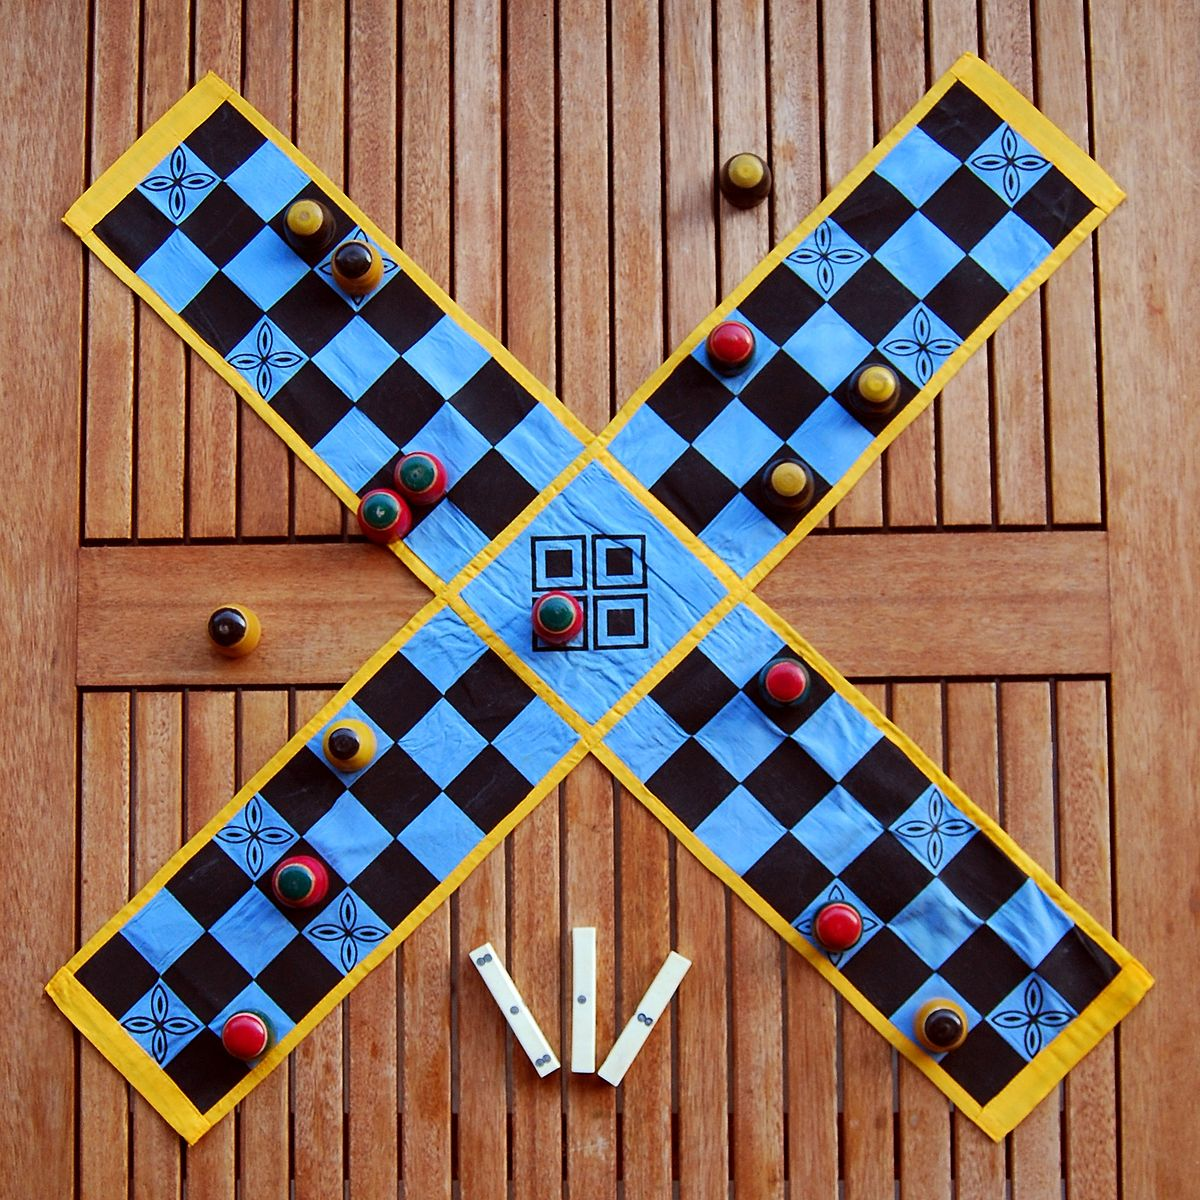
\includegraphics[width=0.4\textwidth]{images/pachisi.jpg}}
    \caption{Pachisi}
\end{figure}
Mittlerweile existieren auch einige Abk\"ommlinge und Varianten mit ver\"anderten Regeln oder Spielfeldern. Allen Varianten ist jedoch gemein, dass sie ein symmetrisches Spielfeld besitzen und analog entwickelt wurden. Man kann vermuten, dass mit asymmetrischen Spielfeldern experimentiert, dies jedoch
nicht weiter verfolgt wurde, da es ungleich schwieriger ist, eine asymmetrische Konfiguration zu finden, bei der die Chancengleichheit und somit der ausgewogene
Spielspass f\"ur alle Spieler gegeben ist. Dennoch ist der Reiz dieses Szenarios nicht zu verachten, da die Freiheit bei der Gestaltung asymmetrischer Spielfelder
\"au\ss erst fruchtbar f\"ur die Entwicklung interessanter Spielvarianten, welche sich nicht in das relativ starre klassische Korsett einpassen m\"ussen, ist. Die gr\"o\ss te
H\"urde in diesem Bereich ist also die m\"uhelose Erstellung eines experimentellen Spielfeldes, um dieses unmittelbar auf seine Spielspa\ss eigenschaften zu testen.
\\\\
Zu diesem Zweck wurde eine Java-Applikation entwickelt, welche einen Spielfeldgenerator implementiert, der mittels einer DSL variable Spielfelder erzeugen kann. Im Verlauf der Architekturdokumentation wird sowohl auf die Besonderheiten der Implementierung, als auch auf die verwendeten Design-Patterns und den Code-Generierungsansatz eingegangen. Abschlie\ss end wird ein Fazit formuliert, das die Erfahrungen und Ergebnisse zusammenfasst.


\section{Anforderungen an die Applikation}

Grundlegend an die Anforderungen ist die Tatsache, dass das Programm f\"ur Programmierer und Designer gleicherma\ss en benutzbar sein mu\ss. W\"ahrend der Designer sich vollst\"andig auf die Entwicklung interessanter Spielfelder konzentrieren k\"onnen mu\ss, d.h. man kann keine Programmierkenntnisse vom ihm verlangen, darf dies den Programmierer nicht daran hindern, die Applikation weiter zu entwickeln, also
in den Bereichen grafisches Erscheinungsbild, Regeln, K\"unstliche Intelligenz und Spielfeld Ver\"anderungen vorzunehmen. \\\\
Aus diesen Gedanken
heraus haben sich die grundlegenden Anforderungen gebildet.
Die Applikation sollte m\"oglichst unabh\"angig vom Betriebssystem lauff\"ahig sein. Da eine starke Eigenschaft von Java die Portabilit\"at und
Lauff\"ahigkeit auf vielen unterschiedlichen Ger\"aten ist, wurde diese als Entwicklungsprogrammiersprache gew\"ahlt. Dadurch lassen sich auch Abk\"ommlinge
des Prototypen (exemplarisch MobileApp) gut planen und umsetzen. Die verbindende Technologie zwischen Programmierer und Designer ist das ausgereifte
Codegenerierungs-Tool Antlr, welches das $.csv$-Dateiformat von Haus aus beherrscht und f\"ur die programmierkenntnislose Erstellung von Spielfeldern
geeignet ist. Diese Aufstellung des Technologiestacks erlaubt einen wechselseitigen Workflow ohne gro\ss e Unterbrechungen. Der Designer kann
mit der aktuellen Version neue Spielfelder erzeugen oder bereits designte testen und Vorschl\"age zum Regelwerk machen. Der Programmierer
kann solche Feature-Requests umsetzen und einspielen, woraufhin der Designer wieder iterieren kann. Beide kommunizieren also vorrangig
\"uber die Grammatik des Spiels und sind nicht prim\"ar an technische Beschr\"ankungen gebunden. Weiter kann der Programmierer unabh\"angig vom Designer
an der grafischen Erscheinung der View und dem Verhalten der k\"unstlichen Spieler arbeiten. F\"ur den Designer ist eine einfache Bedienung
wichtig, d.h. es wird nur von ihm verlangt mit der View zu kommunizieren um neue Spielfelder zu testen. Weitere Deploy-Prozesse muss er nicht beachten.


\section{Genutzte Design Pattern}
\subsection{MVC}
  F\"ur die Abbildung eines Brettspiels in digitaler Form bietet sich das klassische Model-View-Controller Pattern an.

  Dabei ist zu beachten, das die Dreieckbeziehung im MVC nicht symmetrisch, sondern hierarchisch implementiert wird, da sonst die Verantwortlichkeiten
  von Model, View und Controller aufgeweicht werden und feste Kopplungen sowie Spaghetti-Code beg\"unstigt werden. Konkret bedeutet das, das der Controller das Model und die View kennt, die View jedoch nur, um seine Callbacks auf asynchrone Events (z.B. Benutzereingaben) der View anzumelden. Als Controller darf er im Zuge des Spielablaufs im Model Ver\"anderungen vornehmen. Die View kennt das Model, darf aber nur daraus lesen, um sich selbst, d.h. die grafische Darstellung der Applikation auf dem aktuellsten Stand zu halten. Das Model als Datenhalter kennt niemanden, stellt aber Lese- und Schreibfunktionen zur Verf\"ugung. \\\\
  Diese Aufteilung ist noch weiter ausbauf\"ahig, bei zunehmender Komplexit\"at w\"are es sinnvoll f\"ur die
  Einhaltung der Verantwortlichkeiten das EventDispatcher-Pattern hinzuzuf\"ugen. Dadurch k\"onnen das Model und die View Events bei Eingabeereignissen oder Datenver\"anderungen senden, ohne dass die lose Kopplung verlorengeht. Im Prototypen wurde sich dagegen entschieden, da ein einzelner Aufruf f\"ur die GUI-Aktualisierung pro Spielzug und die Anmeldung zweier Callbacks den Mehraufwand nicht rechtfertigten.

\subsection{Singleton}

Die Applikation soll stets ein lauff\"ahiges Mensch-\"arger-Dich-nicht-Spiel repr\"asentieren, welche aufgrund des Designeraspekts ohne komplizierte Laufzeiteinstellungen auskommen oder Kommandozeilenparametern zu starten sein mu\ss. Es ist also nicht erw\"unscht, das mehrere Instanzen der Hauptklassen erzeugbar sind, da dies zu kompliziertem Initialisierungscode mit entsprechend notwendigen Konfigurationen von au\ss en in den Toplevelschichten f\"uhren w\"urde. Im Code wird dies dadurch reflektiert, dass die Hauptklassen von Model, View und Controller als Singletons implementiert sind. Dies dient au{\ss}erdem der Objektkonsistenz, da sichergestellt wird, das immer nur ein und dieselbe Instanz des Objekts existiert und eine fehlerhafte Referenzierung ausgeschlossen ist.
Die Eleganz dieser Variante zeigt sich in der \"ubersichtlichen \texttt{Main}-Klasse, in der nur noch die Singletons instanziiert und miteinander verkn\"upft werden. S\"amtliche Weiterentwicklung des Programms kann innerhalb der MVC-Komponenten erfolgen, ohne das die \texttt{Main} angepasst werden mu\ss .

\section{Implementierung}
Die Applikation wurde in einem 2er-Team entwickelt. Als erstes wurde die Grammatik definiert, damit dann parallel
ein Grundger\"ust der Applikation $MenschAergerDichNicht$ entworfen und der Generator $MADPlayfieldGenerator$ geschrieben werden konnte. Nachdem beide Projekte minimal lauff\"ahig waren, haben sich die Entwicklungsrollen iterativ vermischt, bis der Prototyp ausreichend angereichert und getestet
war.
\\\\
F\"ur die einfache und konfigurationslose Verkn\"upfung der beiden Projekte wurde ein relativer Pfad, welcher lediglich verlangt, dass sich beide Projekte nebeneinander in einem Ordner befinden und ein fester Name $GEN\_PlayfieldCreator.java$ f\"ur die erzeugte Quellcodedatei gew\"ahlt.
Dadurch konnte die Code-Generierung mit einem einzigen Befehl permanent angewendet werden.

\subsection{Grammatik/DSL}
  Die Grammatik des Spiels enth\"alt Symbole f\"ur alle m\"oglichen Spielfeldtypen und deren Verkn\"upfungen zum Nachfolgefeld.
  Es k\"onnen Spielfelder f\"ur 2 bis 4 Spieler definiert werden. Das reichte f\"ur den Prototyp aus und kann ohne besondere
  Schwierigkeiten erweitert werden. Die Spielfeldtypen eines klassischen Mensch-\"arger-Dich-nicht-Spiels sind wie folgt im Code und in der DSL realisiert:

\begin{table}[h!]
  \centering
  \caption{Tiletypes}
  \label{tab:table1}
  \begin{tabular}{ccc}
    \toprule
    Java & DSL\\
    \midrule
    HOME & H[p]\\
    START & S[p]\\
    GOAL & G[pn] \\
    WAY & W[n] \\
    TOGOAL & W[n]G[n] \\
    NONE & NO \\
    \bottomrule
  \end{tabular}
\end{table}

Das K\"urzel $n$ steht f\"ur die Knoteninformation, welches Feld dem betreffenden folgt, dies kann eine der 4 Himmelrichtungen $N$,$S$,$W$,$E$ sein. Das andere K\"urzel $p$ hingegen enth\"alt die Spielernummer 1-4. Einen kleinen Spezialfall stellt der Typ $TOGOAL$ dar, das dies ein Spielfeldtyp ist, welcher zwei Nachfolgeknoten enth\"alt. Der zweite ist die Abzweigung in die Zielfelder des jeweils passenden Spielers. Durch die knotenbasierte Definition
der Spielfelder ist dies jedoch problemslos implementierbar (siehe Abbildung 4 auf Seite 4) und auch erweiterbar.
Da das $.csv$-Format zeilenbasiert ist, wurde f\"ur den Prototypen entschieden, nur matrixartige Spielfelddefinitionen zuzulassen. Dies wird im unten erkl\"arten \texttt{PlayFieldMetaListener} \"uberpr\"uft.
Die EBNF der Grammatik ist in Abbildung 2 dargestellt. Sie beschreibt die zul\"assigen Symbole innerhalb der $.csv$-Datei und den dazugeh\"origen Separierer, der in diesem Fall ein Semikolon ist. 

\begin{figure}[]
    \centering
    \fbox{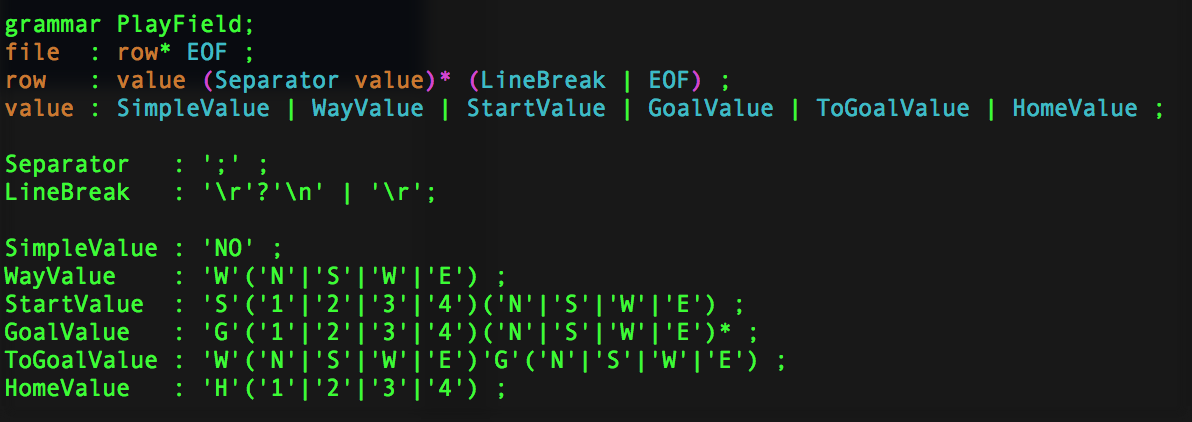
\includegraphics[width=0.45\textwidth]{images/Grammatik.jpg}}
    \caption{Grammatik}
\end{figure}


\subsection{Generator}

Um aus den $.csv$-Dateien eine $.java$-Datei zu erzeugen, musste ein zweistufiges Parsen implementiert werden, welches in
den vorgegebenen Antlr-Java-Code eingeh\"angt wurde. Der erste Parser \texttt{PlayFieldMetaListener} ermittelt Metadaten des Spielfeldes, die der zweite Parser \texttt{PlayFieldSemanticListener} ben\"otigt, um den spielfelderzeugenden Code generieren zu k\"onnen. Dazu wird die $.csv$-Datei einmal durchlaufen um die Metadaten zu akkumulieren. Zu diesen geh\"oren die Anzahl der Spieler, die gleichzahligen Home- und Endpositionen der jeweiligen Spieler, das Vorhandensein genau eines Startfeldes pro Spieler sowie die Anzahl der Zeilen und Spalten der $.csv$-Definition. Etwaige Fehler werden mit einer Abbruchsmeldung quittiert. Sind alle Metadaten gesammelt, was erst nach einem vollst\"andigem Scan garantiert ist, kann der \texttt{PlayFieldSemanticListener} gestartet und ihm die nun vorliegenden Metadaten \"ubergeben werden, um den Code f\"ur die Spielfeldverkn\"upfungen mit den nun ebenfalls bekannten Indizes zu generieren.
Die generierte Datei enth\"alt danach die Zugriffsfunktionen 
\texttt{getNumRows},
\texttt{getNumColumns},
\texttt{getNumPlayers} und
\texttt{getNumPiecesPerPlayer}
f\"ur die Metadaten und die spielfelderzeugende Funktion \texttt{createPlayfield}, welche wie in Abschnitt \texttt{Playfield}: auf Seite \pageref{sec:model_playfield} beschrieben benutzt werden. Wie man an einer beispielhaften Zeile\newline
\texttt{playfield.getTile(0, 6)}\newline
\texttt{.setType(TileType.START)}\newline
\texttt{.setNext(playfield.getTile(1, 6))}\newline
\texttt{.setPlayerID(2);}\newline
 innerhalb dieser Methode sehen kann, werden die matrixartige Struktur der $.csv$-Datei und die gewonnenen Metadaten verwendet, um die Knotenverkn\"upfungen zwischen den einzelnen Spielfeldern zu erstellen. Nach dieser Zuordnung kann auf die Koordinatenwerte der Felder vollst\"andig verzichtet werden. Die so generierte Datei enth\"alt die Methoden \texttt{getNumRows}, \texttt{getNumColumns}, \texttt{getNumPlayers} und \texttt{getNumPiecesPerPlayer} mit den ermittelten Daten des Meta-Parsers
sowie die Methode \texttt{createPlayfield} des Semantic-Parsers, welcher eine zu bef\"ullende \texttt{Playfield} Instanz \"ubergeben wird.


\subsection{Applikation}

  Im folgenden werden die einzelnen Klassen der Applikation vorgestellt.\\

\subsubsection{Controller}
\begin{figure}[]
    \centering
    \fbox{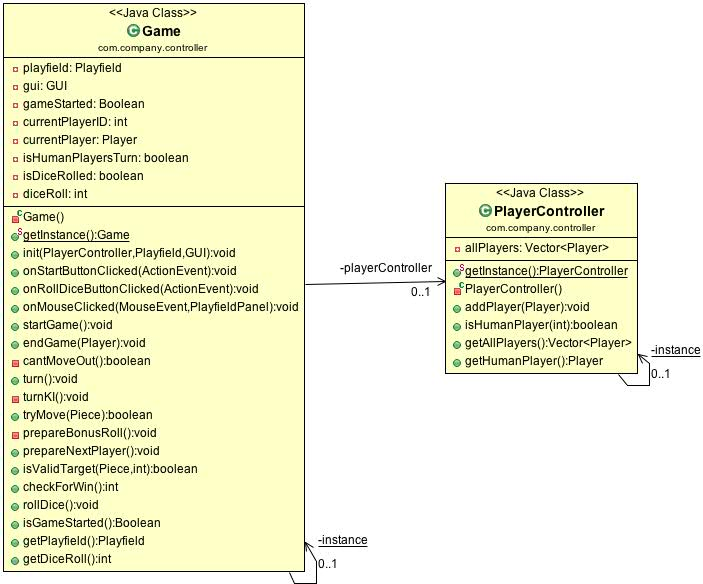
\includegraphics[width=0.47\textwidth]{images/controllerClassDiagram.jpg}}
    \caption{Controller Klassendiagramm}
\end{figure}

Die Klasse \texttt{Game} ist das Herz der Applikation. Als Hauptcontroller h\"alt er Referenzen zum Subcontroller \texttt{PlayerController}, zur View \texttt{GUI} und zum Model \texttt{Playfield}. In der \texttt{Main}-Methode wird die Applikation \"uber\newline
\texttt{Game game = Game.getInstance();}\newline
\texttt{game.init(playerController, playfield, gui);}\newline
zusammengesetzt. Im \texttt{Game}-Controller finden sich die Methoden zur Eingabebehandlung, mit \texttt{onStartButtonClicked} kann ein neues Spiel begonnen werden, mit \texttt{onRollDiceButtonClicked} wird W\"urfeln der menschlichen Spieler verarbeitet und mit \texttt{onMouseClicked} werden Klicks auf das Spielfeld verarbeitet. Dabei handelt es sich um Spielfigurbewegungen der menschlichen Spieler.

Zum Steuern des Spielablaufs existieren die Methoden \texttt{startGame}, mit der ein neues Spiel initialisiert wird.
Die Methode \texttt{checkForWin} pr\"uft nach jedem Spielzug, ob ein Sieger feststeht und beendet gegebenenfalls das Spiel durch
\texttt{endGame}.
Die Methode \texttt{turn} leitet einen Spielzug ein. Im Falle eines menschlichen Spielers wird anschlie\ss end auf Eingaben gewartet, bei einem k\"unstlichen Spieler wird das W\"urfeln automatisch ausgef\"uhrt und die KI \"uber \texttt{turnKI} zur Spielfigurenbewegung angesteuert. Die zufallsgenerierten W\"urfelwerte
werden von \texttt{rollDice} zur\"uckgegeben. F\"ur die Logik innerhalb des Spielablaufs existieren die Methoden
\texttt{prepareBonusRoll}, welche gesondert nach einer gew\"urfelten 6 angesteuert wird und im Falle einer anderen gew\"urfelten Zahl
\texttt{prepareNextPlayer}, wenn der entsprechende Spieler seinen Zug abgeschlossen hat.\\
Die zentrale Methode \texttt{tryMove} wird ausgef\"uhrt, wenn eine Spielfigur von einem Spieler, gleichg\"ultig ob menschlich oder nicht, bewegt werden soll. In ihr werden die Regeln zur validen Bewegung der Spielfigur \"uberpr\"uft, der Zug wenn m\"oglich ausgef\"uhrt (wodurch sich das Model \"andert) und die Validit\"at als \texttt{boolean} Wert zur\"uckgegeben. Durch den R\"uckgabewert wird gesteuert, ob im Falle einer KI eine andere Spielfigur bewegt oder wieder auf Mauseingaben des Benutzer gewartet werden soll. War der Zug valide, wird zum n\"achsten Spieler im Spielverlauf weitergegangen. Unterfunktionen von \texttt{tryMove} sind \texttt{cantMoveOut}, welche die Zwangsregel, dass man eine Spielfigur -wenn m\"oglich- heraussetzen muss und
\texttt{isValidTarget}, welche \"uberpr\"uft, ob das Zielfeld einer Spielfigur ein valide Position darstellt.

Auf die letztgenannte Methode soll kurz genauer eingegangen werden, da sich in ihr die Vorteile des knotenbasierten Spielfeldes zeigen. Zum Ermitteln eines legales Spielzugs der Spielfigur wird zuerst das Feld, auf dem die Spielfigur sich befindet, referenziert und nachfolgend die Methode \texttt{getTargetTile} auf dem referenzierten Spielfeld aufgerufen, dessen Implementierung in Abbildung 4 zu sehen ist. Mithilfe der Nachfolgeknoteninformation wird solange der n\"achste Knoten referenziert, bis entweder kein Nachfolgeknoten existiert (im Falle des letzten Zielfeldes eines Spielers) oder die gew\"urfelte Schrittweite erreicht ist.
Zu beachten ist, dass keinerlei planaren Positionsinformationen ben\"otigt werden. Dadurch ist es m\"oglich, Wege durch v\"ollig frei gestaltete Spielfelder
zu suchen. Weiterhin lassen sich zwanglos neue Spielfeldtypen f\"ur exotischere Spielvarianten hinzuf\"ugen.\\\\
\begin{figure}[]
    \centering
    \fbox{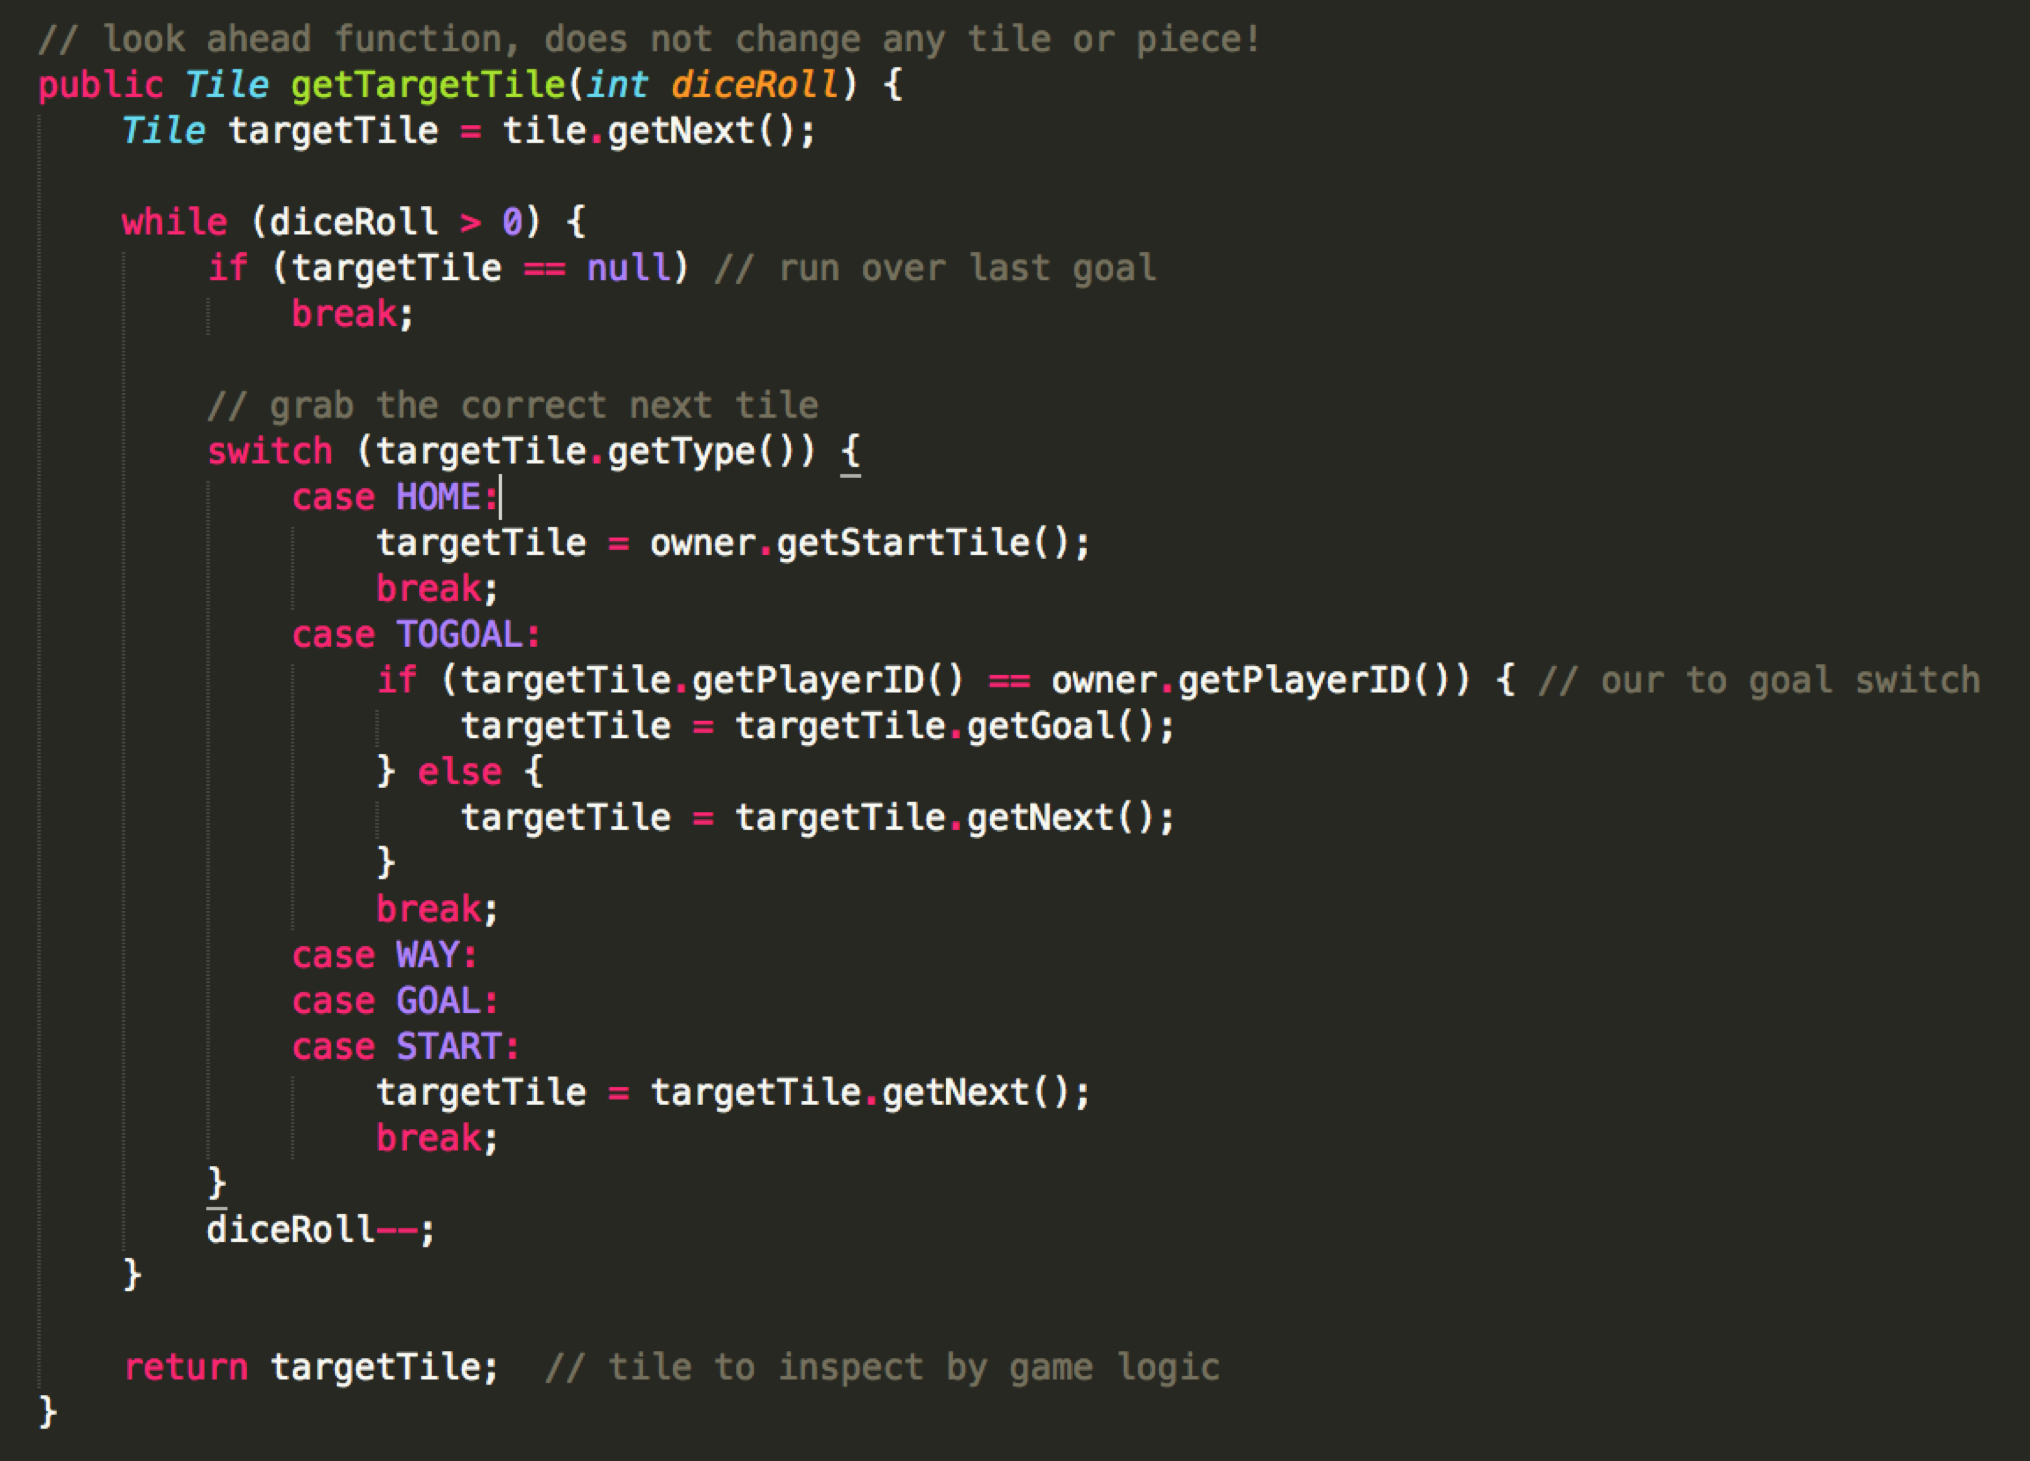
\includegraphics[width=0.47\textwidth]{images/dev.png}}
    \caption{Methode \texttt{getTargetTile}}
    \label{gtt}
\end{figure}
Der \texttt{PlayerController} dient lediglich der Verwaltung der Spieler. Durch diese zus\"atzliche Kapselung wird jedoch der \texttt{Game}-Controller
nicht unn\"otig mit spielablauffremden Methoden aufgebl\"aht, wenn die Spielerverwaltung durch erweiterte Spielmodi komplizierter wird. Dazu geh\"ort beispielsweise die Anmeldung der Spieler (menschlich oder k\"unstlich) beim Spielstart und die sp\"atere Abmeldung f\"ur Spielmodi mit mehreren Siegerpl\"atzen.\\

\subsubsection{View}
\begin{figure}[]
    \centering
    \fbox{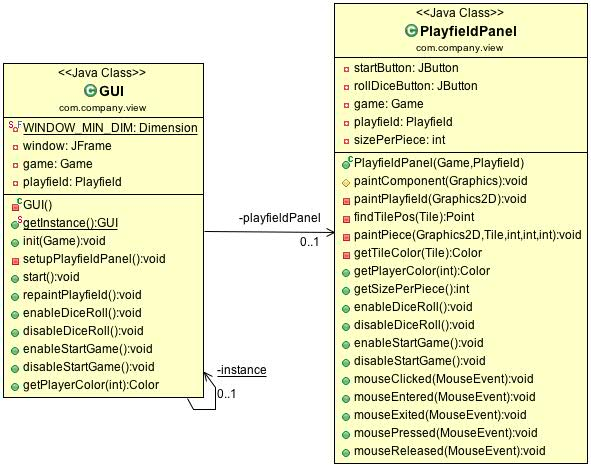
\includegraphics[width=0.47\textwidth]{images/viewClassDiagram.jpg}}
    \caption{View Klassendiagramm}
\end{figure}

Der implementierte Singleton \texttt{GUI} repr\"asentiert das generierte Mensch-\"arger-Dich-nicht-Spielfeld. Es besteht aus einem \texttt{PlayfieldPanel}, welches f\"ur die Darstellung von \texttt{JPanel} erbt und f\"ur die Interaktion mit dem Nutzer den MouseListener implementiert. Das \texttt{PlayfieldPanel} stellt die einzelnen \texttt{Tile}s, also Felder, mittels zur Laufzeit gerenderten Kreisen dar. Diese Kreise k\"onnen wei{\ss} f\"ur normale Wegfelder und farbig f\"ur Felder eines Spielers sein. \\
  Die einzelnen Figuren der Spieler werden als kleinere Kreise innerhalb des Feldes dargestellt und durch die Nutzung von \texttt{.darker()} als separate Spielfigur visualisiert. f\"ur die Steuerung des Spiels stehen Buttons zum ausl\"osen des Wurfs und zum Starten des Spiels zur Verf\"ugung. Au{\ss}erdem kann durch Klick auf eine der eigenen Spielfiguren eine Bewegung um die gew\"urfelte Augenanzahl ausgel\"ost werden. Auf alle diese asynchronen Aktionen sind die vorher beschriebenen Callbacks des \texttt{Game}-Controllers angemeldet. Die Klasse \texttt{GUI} stellt das Fenster und alle n\"otigen Delegationsmethoden zur Steuerung des \texttt{PlayfieldPanel} zur Verf\"ugung. \\

\subsubsection{Model}
\begin{figure}[]
    \centering
    \fbox{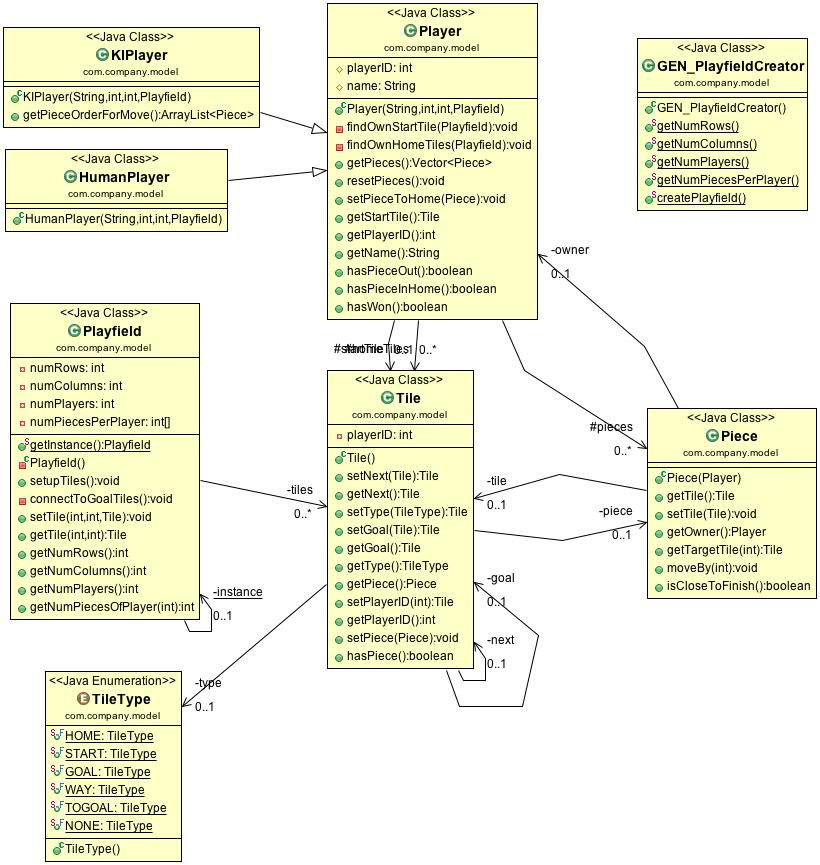
\includegraphics[width=0.47\textwidth]{images/modelClassDiagram.jpg}}
    \caption{Model Klassendiagramm}
\end{figure}

Das Modell hinter dem Spiel beschreibt sowohl die Repr\"asentation des Spielfelds, als auch die beiden Spielertypen \texttt{HumanPlayer} und \texttt{KIPlayer} sowie die Spielfiguren. Das Spielfeld besteht aus beliebig vielen \texttt{Tile}s, die die einzelnen Spielfelder repr\"asentieren. Da die \texttt{Tile}s eine Typeigenschaft besitzen, kann ein eleganter Regelwerk-Code implementiert werden, der eine variable Spielfeldbeschaffenheit und eine einfache Erweiterung der Regeln erm\"oglicht.
Im folgenden wird genauer auf die einzelnen Modellklassen eingegangen.\\

\texttt{Player}: Die Klasse \texttt{Player} ist die Basisklasse aller Spieler und besitzt Grundinformationen wie z.B. die \texttt{playerID} und den Spielernamen. Au{\ss}erdem kennt die \texttt{Player}-Klasse die Spielfiguren und somit auch die Information, auf welcher \texttt{Tile} des Spielfeldes sich die Spielfigur befindet. Anhand des im Konstruktor \"ubergebenen \texttt{Playfield}s findet eine Auswertung der $START$- und $HOME$-Felder statt. Die Klassen \texttt{KIPlayer} und \texttt{HumanPlayer} erben von \texttt{Player} und differenzieren, ob der Zug automatisch ausgef\"uhrt werden soll, oder ob auf die Reaktion des Spielers gewartet werden muss. \\

\texttt{Piece}: Die Klasse \texttt{Piece} repr\"asentiert eine Spielfigur eines Spielers. Ein \texttt{Piece} geh\"ort immer zu einem \texttt{Player} und steht auf einem \texttt{Tile}. Mittels der Methode \texttt{getTargetTile}, die bereits in der Klasse \texttt{Game} beschrieben ist und der Methode \texttt{moveBy} kann die Spielfigur um die gew\"urfelte Anzahl eines Spielzuges bewegt werden. Au{\ss}erdem kann durch die Methode \texttt{isCloseToFinish} ermittelt werden, ob sich die Spielfigur in der Reichweite des Ziels befindet. \\

\label{sec:model_playfield}
\texttt{Playfield}: Die Klasse \texttt{Playfield} dient der Verkn\"upfung der codegenerierten Spielfelder und der \texttt{GUI}. Hier ist die Code-Generierungsklasse \texttt{MAD\_PlayfieldCreator} inkludiert und wird im Konstruktor der \texttt{Playfield}-Klasse aufgerufen. Damit die \texttt{Tile}s automatisch bef\"ullt werden k\"onnen, besitzt die \texttt{Playfield}-Klasse die Methode \texttt{setupTiles}, welche von der generierten Klasse aufgerufen wird. Anschlie\ss end ruft \texttt{Playfield} noch ihre Methode \texttt{connectToGoalTiles} auf, um die speziellen $TOGOAL$-\texttt{Tile}s mit den passenden
$GOAL$-Feldern zu verkn\"upfen. Au{\ss}erdem kennt sie durch die generierte Klasse die Anzahl der Reihen, Spalten, Spieler und Spielfiguren pro Spieler und bietet f\"ur die Controller Delegationsmethoden an.\\

\texttt{Tile}: Die Klasse \texttt{Tile} speichert die Knoten- und Referenzinformationen der Spielfiguren des Spielfelds. Eine Instanz der Klasse \texttt{Tile} besitzt Informationen \"uber den \texttt{TileType}, die Spielfigur die eventuell mit ihr assoziiert ist und die \texttt{playerID}. Des weiteren verf\"ugt sie \"uber die Information, welche \texttt{Tile} ihr Nachfolger ist und ggf. ob es eine \texttt{Tile} ist, die sich vor einer Ziel-\texttt{Tile} befindet. \\
\begin{figure}[]
    \centering
    \fbox{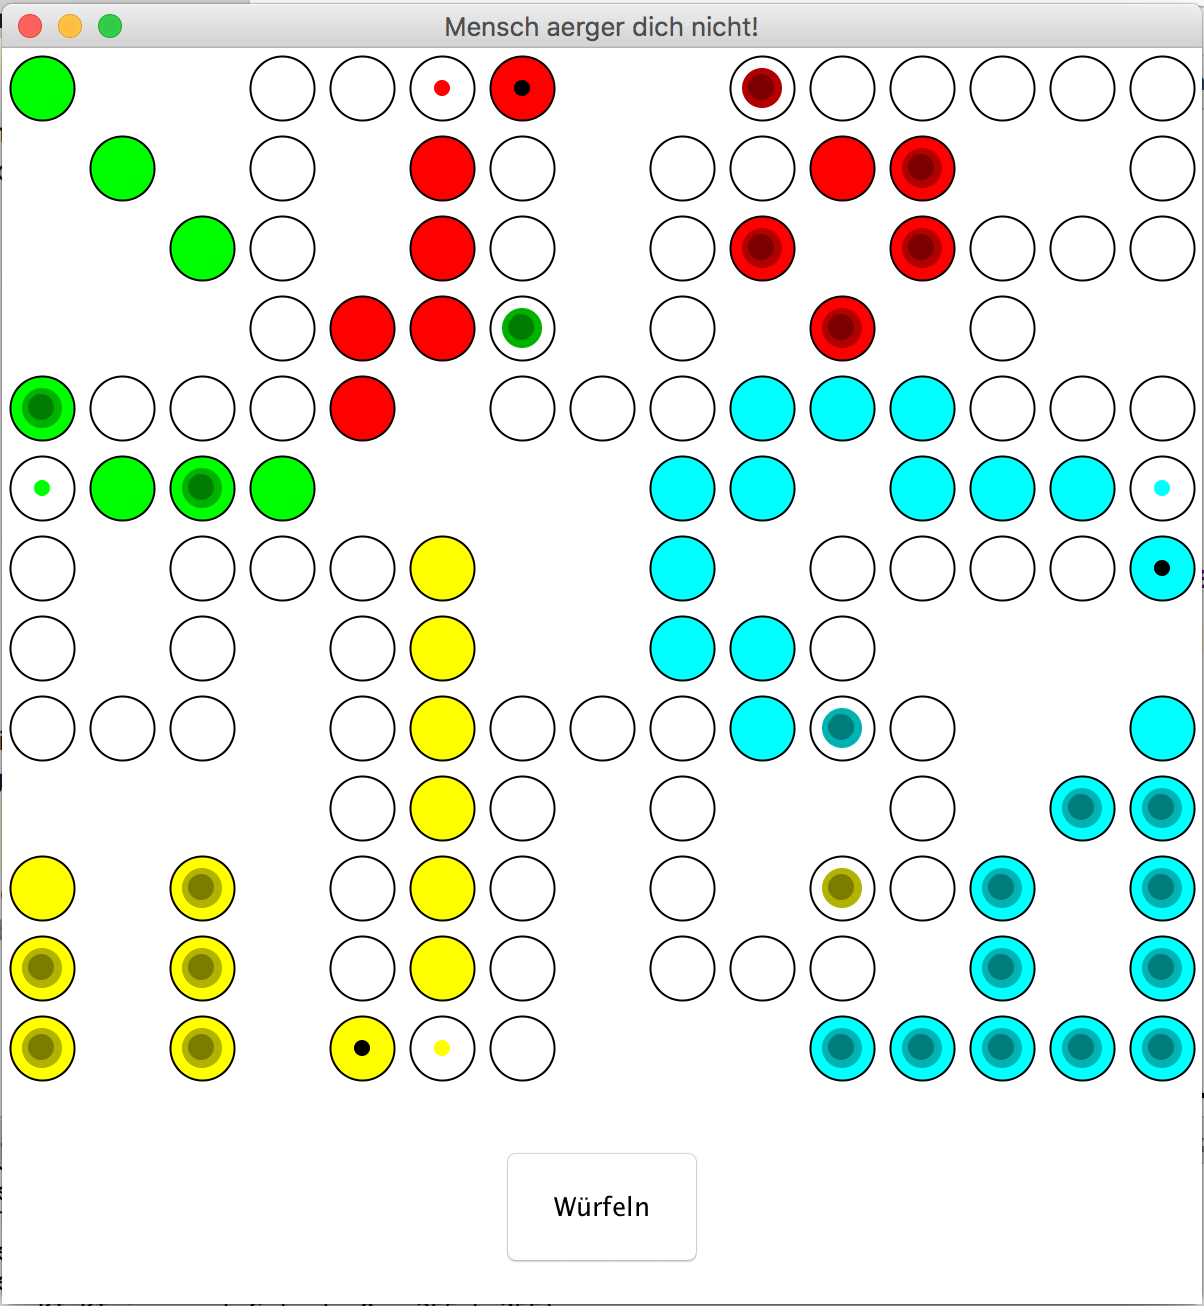
\includegraphics[width=0.47\textwidth]{images/gui.jpg}}
    \caption{GUI}
\end{figure}
\\\texttt{TileType}: Die Enumeration \texttt{TileType} beschreibt den Typ eines \texttt{Tile}-Objekts. Die m\"oglichen Typen sind: $HOME$ f\"ur ein Hausfeld, $START$ f\"ur ein Startfeld, $GOAL$ f\"ur ein Zielfeld, $WAY$ f\"ur ein Wegfeld, $TOGOAL$ f\"ur ein Feld, das sich vor einem Zielfeld befindet und $NONE$ f\"ur eine nicht spielrelevante \texttt{Tile}. \\

\section{Fazit}

Aufgrund der relativ kurzen Entwicklungszeit mussten beim urumf\"anglichen Architekturdesign Abstriche gemacht werden.
Dennoch wurde darauf geachtet, dass die beschnittenen Teile so ausgelegt wurden, dass eine sp\"atere Erweiterung
ohne grosses Refactoring m\"oglich ist, beispielsweise seien hier die direkt verkn\"upften Callbacks statt eines ausgewachenen EvenDispatcher-Pattern oder der \texttt{PlayerController} genannt. Das Ziel, einen stabilen Prototypen f\"ur dynamische Mensch-\"arger-Dich-nicht-Spielfelder zu programmieren, wurde erreicht. Die feste Schnittstelle in der \texttt{Playfield}-Klasse zum generierten Code hat sich als \"ausserst fruchtbar f\"ur den unterbrechungslosen Workflow in den Bereichen Grammatik-, Spielregel- und Grafikerweiterung herausgestellt. Die Umwandlung von zeilen- und spaltenbasierten Informationen in eine Knotenstruktur hat wesentlich zu elegantem und intuitivem Code gef\"uhrt und entkoppelt die grafische Darstellung von der Semantik des Spielfeldes. Im Verlauf der Entwicklung hat sich herauskristallisiert, dass f\"ur Spielfelder, die grafisch noch wesentlich freier gestaltbar sein sollen, so z.B. geschwungene Wege oder Felder mit mehr als 3 Knotenverkn\"upfungen, die Grammatik jedoch genauestens \"uberdacht werden sollte. Eine Kl\"arung dieser Fragestellungen ist nach den Erfahrungen dieses Prototypen der richtige Weg f\"ur Refactorings und Workflowprozesse in den verschiedenen Bereichen der Applikation. F\"ur eine komplette Worksuite zur Herstellung von Spielvarianten vorstellbar sind ein grafischer Spielfeldeditor, welcher die dann komplizierteren Grammatiken f\"ur den Designer erzeugen kann sowie weitere Code-Generatoren im Bereich von k\"unstlichen Mitspielern und abweichenden Spielregels\"atzen. Abschlie{\ss}end l\"asst sich sagen, das der anf\"angliche Mehraufwand, einen relativ aufw\"andigen Parser zu schreiben, in der sp\"ateren Phase des Projektes beim Testen, Debuggen und Weiterentwickeln mehr als gelohnt hat. Eine manuelle Bearbeitung von Java-Code, um neue Spielfeldkombinationen zu testen, w\"are entwicklungstechnisch untragbar gewesen.

\end{document}


